\section{General-purpose Counterfactuals}
\label{sec:general_purpose}



\newcommand{\tagdefine}[1]{\emph{{\color{darkgray}#1} }}
%\renewcommand{\arraystretch}{1.1}
\newcommand{\TagTable}{
\begin{table*}
\small
\centering
\begin{tabular}{@{} p{0.11\linewidth} p{0.61\linewidth}  p{0.22\linewidth} @{}}
\toprule
\textbf{\Tagstr} & \textbf{Definitions and \sysname-generated Examples} & \textbf{Training datasets} \\ 
\midrule
\ctrltag{negation}
    & A dog is \add{not} embraced by the woman.
    & \cite{kaushik2019learning}
\\ \midrule
\ctrltag{quantifier}
    & \swap{A dog is}{Three dogs are} embraced by the woman. 
    & \cite{gardner2020contrast}
\\ \midrule
\ctrltag{shuffle}
    & \tagdefine{To move (or swap) key phrases or entities around the sentence.} \newline
    A \swap{dog}{woman} is embraced by the \swap{woman}{dog}.
    & \cite{zhang2019paws}
\\ \midrule
\ctrltag{lexical}
    & \tagdefine{To change just one word or noun chunks without breaking the POS tags.} \newline
      A dog is \swap{embraced}{attacked} by the woman.
    & \cite{sakaguchi2019winogrande}
\\ \midrule
\ctrltag{resemantic}
    & \tagdefine{To replace short phrases or clauses without affecting the parsing tree.}\newline
      A dog is \swap{embraced by the woman}{wrapped in a blanket}.
    & \cite{wieting2017paranmt}
\\ \midrule
\ctrltag{insert}
    & \tagdefine{To add constraints without affecting the parsing structure of other parts.} \newline
      A dog is embraced by the \add{little} woman.
    & \cite{mccoy2019right}
\\ \midrule
\ctrltag{delete}
    & \tagdefine{To remove constraints without affecting the parsing structure of other parts.} \newline
    A dog is embraced \remove{by the woman}.
    & \cite{mccoy2019right}
\\ \midrule
\ctrltag{restructure}
    & \tagdefine{To alter the dependency tree structure, \eg changing from passive to positive.} \newline
    A dog is \swap{embraced by}{hugging} the woman.
    & \cite{wieting2017paranmt}
\\
\bottomrule
\end{tabular}
\vspace{-5pt}
\caption{A list of \tagstrs used for semantically driving the counterfactual generation in \sysname, their examples, and the representative training datasets for the corresponding patterns. %More examples are in Appendix~\ref{appendix:example}.
}
%\wts{Change all the examples to be on an identical sentence, not all different cases. And consider further annotate the tags based on whether they just do semantic change or also syntactic change.}}
\label{table:ctrltag}
\vspace{-10pt}
\end{table*}
}
% on a particular instance
% 
\subsection{Definition and Desiderata}
\label{sec:desiderata}


Given an instance $x \in \xset$, a generator $g$ should produce a set of counterfactuals $\hat{\xset} = \{\xp_1, \xp_2, ...\}$ with various relationships $x \veryshortarrow \xp_i$ (referred as $\relation{\xp_i}$ for simplicity).
% Each $\xp_i$ perturbs $x$ with certain strategies like negations, syntactic restructuring, etc., and the edited spans are instantiations of the strategies.
For example, \swap{great}{not great}, \swap{kids}{no one} in Figure~\ref{fig:teaser}B are both instances of the \ctrltag{negation} relationship.
The importance of certain $\relation{\xp}$ changes along with applications.
The two negation changes also invoke a \emph{label flipping relationship} for sentiment analysis, with both counterfactuals becoming negative sentences; however, this relationship does not necessarily hold for another task.
However, \emph{independent of the application}, we prefer $\xp$ with the following four desiderata, \ie closeness, fluency, diversity, and controllability:
%which inspire our modeling in \S\ref{subsec:nlg}:
% Knowledge of such relationships aid downstream filtering and ranking.
% $\relation{\xp}$ then forms certain relationships that are useful for downstream filtering (\eg perturbation strategy, the added and removed tokens, the impacts on groundtruth label, model prediction, etc.)
%The perturbation follow certain \emph{strategies} $s$ (e.g., negations~\cite{kaushik2019learning}, word substitution~\cite{li-etal-2020-bert-attack}, syntactical restructing~\cite{iyyer2018adversarial}).

%Desired counterfactuals are usually~\cite{morris2020textattack}:
Considering \emph{individual counterfactuals}, a $\xp$ should be (1) \textbf{close} to $x$, preferably only involving the minimal changes necessary for establishing a certain effect while leaving the rest of the instance intact~\cite{pearl2018causal}, such that users can make causality assessments from $\relation{\xp}$. 
%If we add negation \emph{and} remove a clause from a particular $x$ simultaneously, it is unclear which change should the resulting behavior be attributed to. 
It has long been observed that humans strongly favor counterfactuals that are closer to the original instance~\cite{kahneman}.
%, even when the same variable is acted upon.
%Following common practice in NLP research, we estimate \emph{closeness} using the semantic and syntactic distance between $x$ and $\xp$~\cite{morris2020textattack, madaan2020generate}.
However, $\xp$ also needs to be (2) \textbf{fluent}, \ie grammatically correct~\cite{morris2020textattack} and semantically meaningful (\eg \exinline{It's scary for water} is not meaningful.)
This estimates the likelihood of a sentence occurring in reality; as \citet{kahneman} stated, the counterfactual scenario should be one that could have easily happened without rare assumptions. 
%In NLP, this translates to sentences that are likely to be written.


%However, $\xp$ also needs to be realistic, \ie the counterfactual scenario should be one that could have easily happened, without rare assumptions or coincidences~\cite{kahneman}. 
%In NLP, this translates to sentences that are likely to be written, \ie (2) \emph{fluent} counterfactuals that are grammatically correct~\cite{morris2020textattack} and semantically meaningful (\eg \exinline{It's scary for water} is grammatically correct but not meaningful.) 

We also consider \emph{sets of counterfactuals}, as there can be infinite numbers of ``what-ifs''~\cite{pearl2018causal}. %especially as we allow $\xp$ to deviate from $x$. 
Since our goal is to produce a general-purpose set of counterfactuals, we expect the set to be (3) \textbf{diverse} in terms of relationships between $x$ and $\xp$.
%However, when the targeted relationship is unclear, an approximation could be the similarity of counterfactuals \emph{to each other} (using \eg self-BLEU~\cite{Hu2017TowardCG}).
%, and also to contain various instantiations of the same relationship.
Meanwhile, we also expect to collect sets with (4) \textbf{controlled} $\relation{\xp}$ relationship.
The control is essential to support a wide range of specific applications, \eg counterfactual explanations on salient features (\S\ref{sec:app_explain}), error analyses that group semantically or syntactically related $\xp$ (\S\ref{sec:app_err_analysis}), etc.
It reflects the ``focus rule''~\cite{kahneman}: counterfactuals would vary with the object of attention.
%Additionally, augmentations usually prioritize (3) \emph{diversity} --- a group of $x$s are preturbed using various strategies, and various initiations under the same strategy, such that they provide different constraints on finetuning decision boundaries.
%On the other hand, evaluations and explanations require more (4) \emph{controlled} perturbations for systematic and targeted inspections.
%The diversity and the controllability are two competing factors, and prior work focusing on certain applications follow one of two extremes.
%Those that thrive in diversity are either too uncontrolled (\eg text generation~\cite{iyyer2018adversarial}) or hard to scale (\eg manual rewrites~\cite{kaushik2019learning, gardner2020contrast}), whereas those that rely on templates or heuristic rules usually only cover limited linguistic patterns~\cite{li2020linguistically}.





\subsection{Modeling through Text Generation}
\label{subsec:nlg}

We frame counterfactual generation as a text generation task using language models (LMs).
Large pre-trained LMs like GPT-2~\cite{radford2019language} are capable of generating \emph{fluent} text.
They also increase the semantic and syntactic \emph{diversity}, by allowing for non-trivial countrefactuals that are more flexible than word substitutions~\cite{garg2019counterfactual} and templates~\cite{ribeiro2018sear}. 




\begin{figure}[t]
\centering
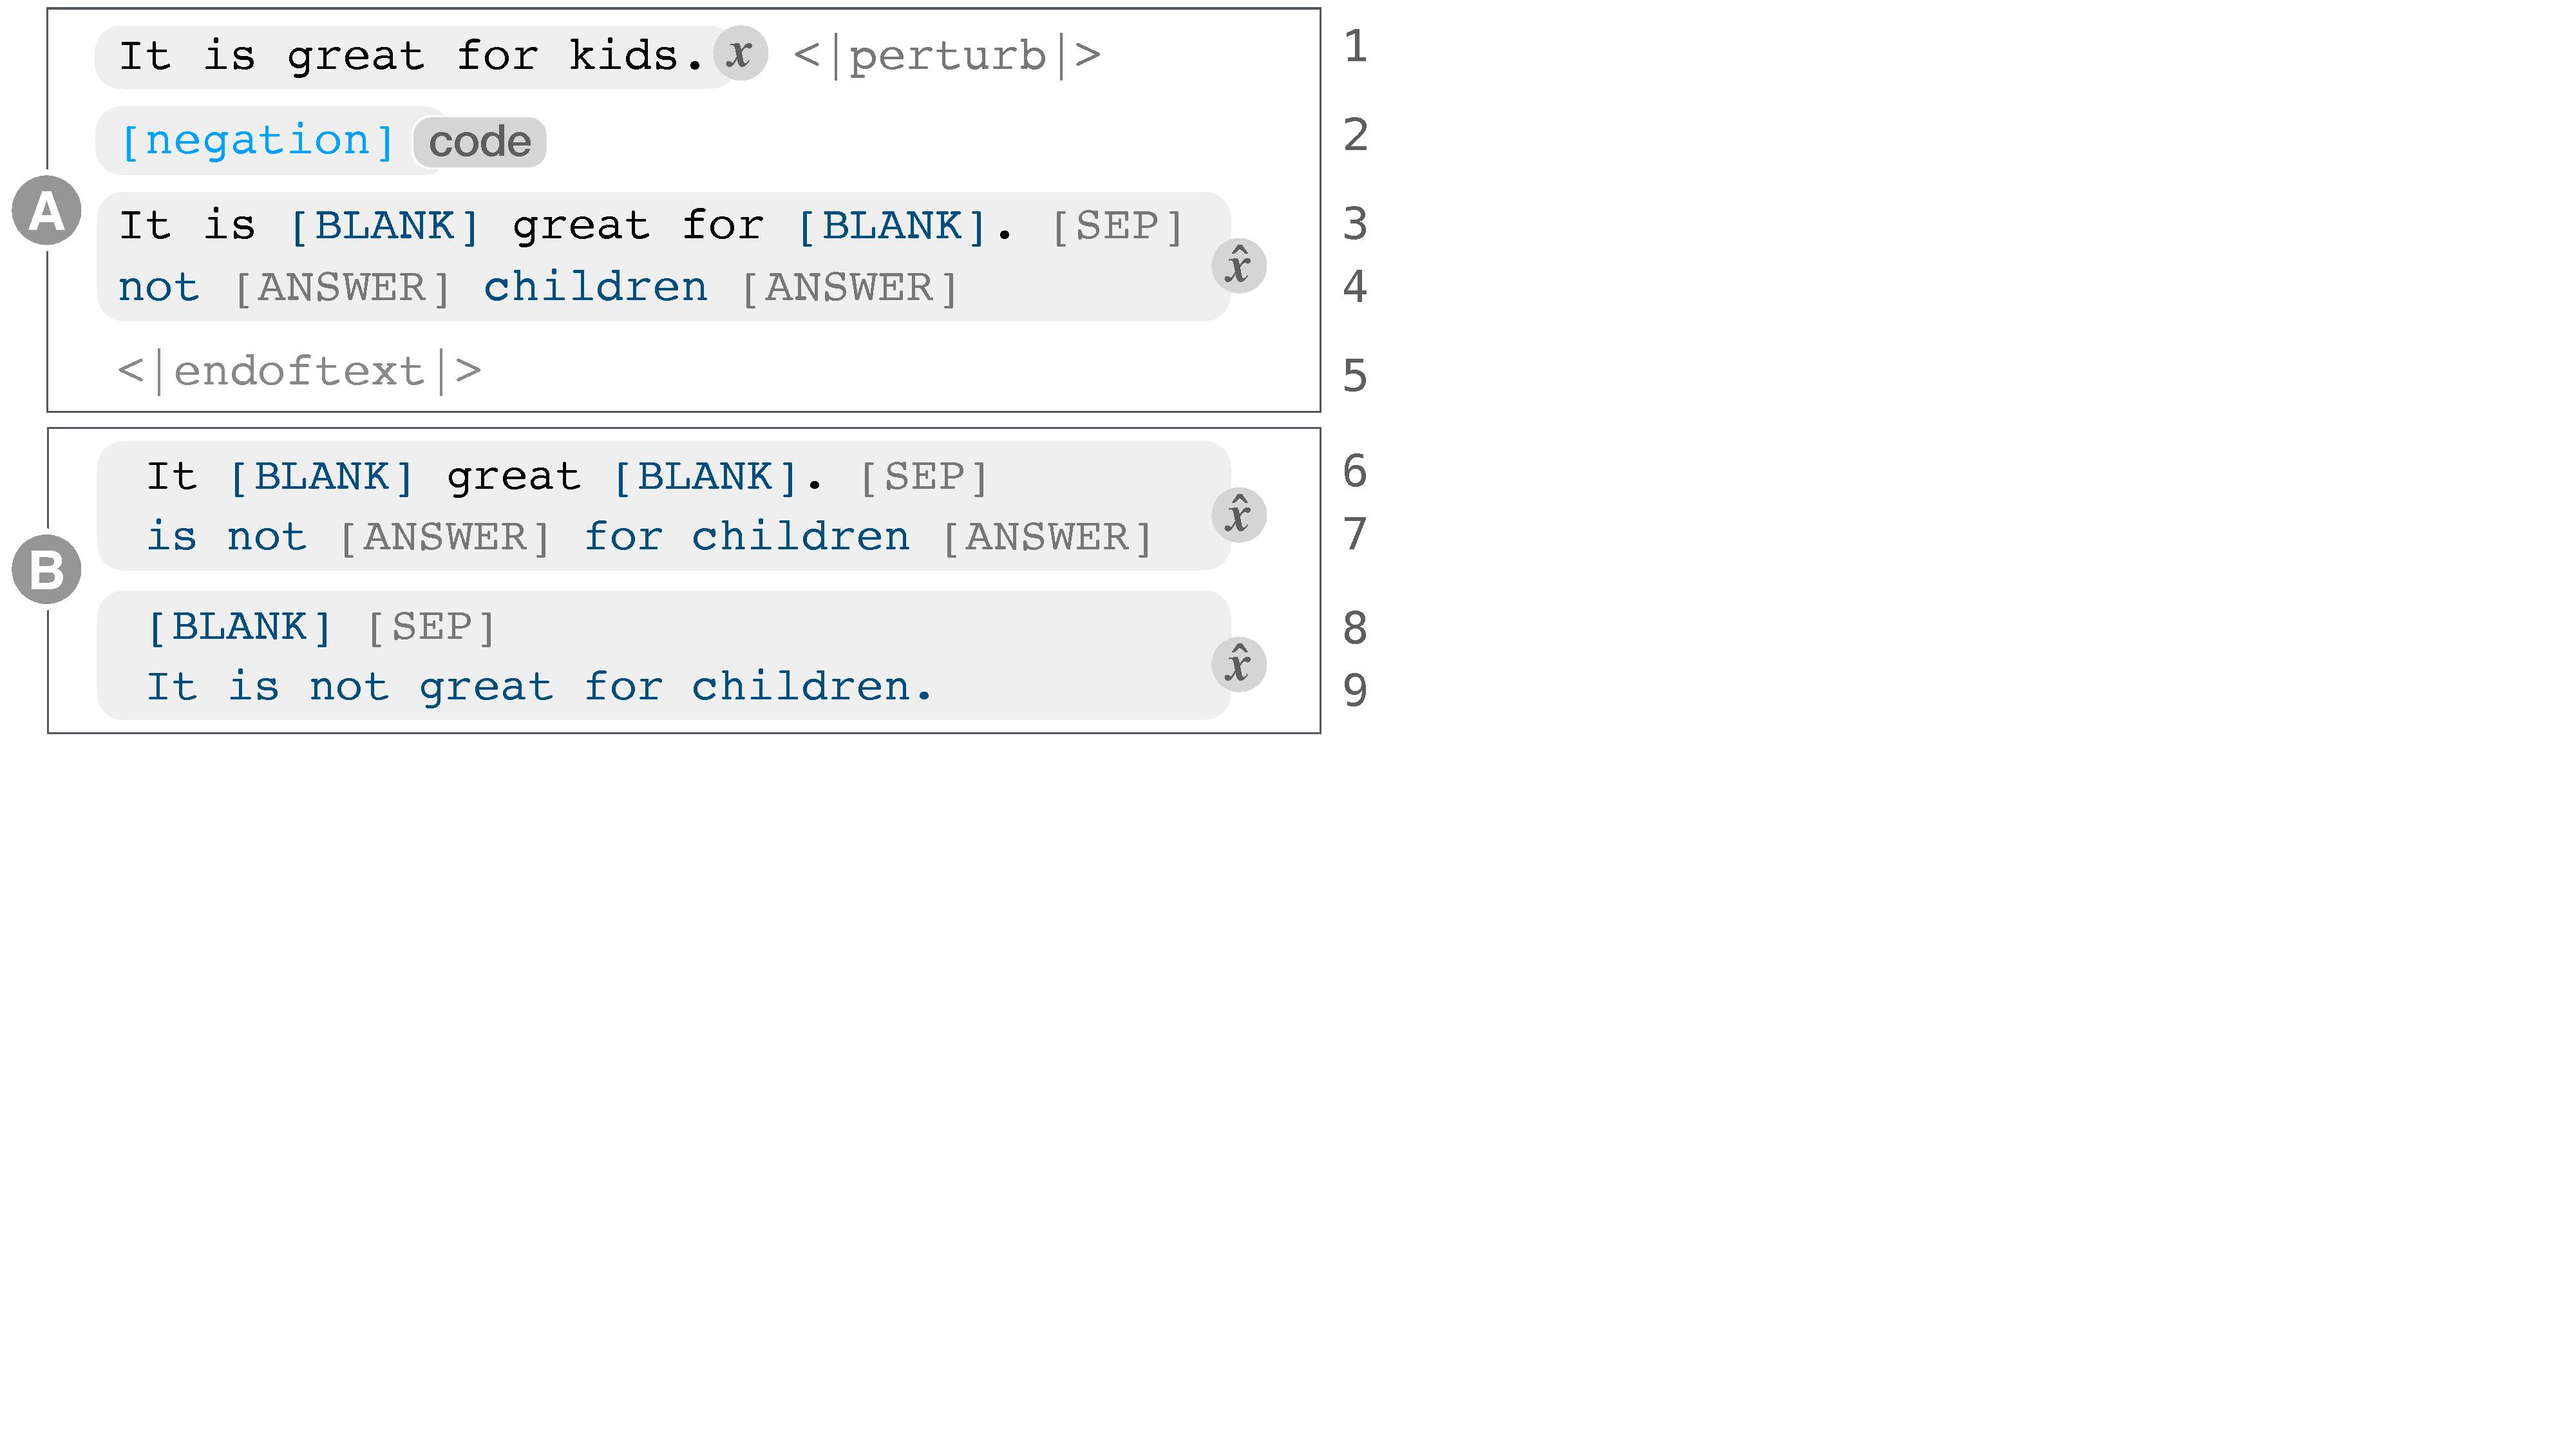
\includegraphics[trim={0 18.8cm 31cm 0cm}, clip, width=1\columnwidth]{figures/blank.pdf}
\vspace{-15pt}
\caption{  
(A) The text format for \sysname, which concatenates the original $x$, the \tagstr, and the $\xp$ (converted to the infilling structure from \exinline{It is not great for children}).
At \emph{generation} time, \sysname accepts prompts that just include $x$ (Line 1), or with the \tagstrshort and the \texttt{BLANK}s (Line 2--3).
During training, the \tagstrshorts and blanks are automatically extracted.
(B) The blanking structure can flexibly cover just the $\xp$ subtrees that contain the change, or the entire sentence, such that Line 3--4 in (A) can be replaced by Line 6--7 or 8--9.
%We get multiple training texts per pair, by blanking $\xp$ subtrees that contain the change, or the entire sentence.
}
\vspace{-10pt}
\label{fig:blank}
\end{figure}



\paragraph{Overview: the text prompt format.}
As shown in Figure~\ref{fig:blank}A, at generation time, the input prompt to \sysname \emph{always} starts with $x$, followed by a special token (Line 1).
This ensures that the generated $\xp$ are conditioned on, and \emph{close to} an original $x$, rather than arbitrary text.
The generation can also be conditioned on \emph{\tagstrs} (Line 2), which encodes the type of change, and \texttt{BLANK} \emph{tokens} (Line 3), which encodes where the change happens.
These two encodings help achieve control over $\relation{\xp}$, such that \sysname only needs to fill in the blanks sequentially according to the controls (Line 4).
Note that the control conditions are optional.
When we exclusively condition the generation on $x$ (Line 1), \sysname can generate Line 2--3 on its own by selecting the \tagstr and the location of blanks.
Next, we detail how we finetune GPT-2 to insert such formats.

\TagTable

\paragraph{\emph{Closeness} and \emph{Controllability}: Using \tagstrs and infilling structures.}
To build the close mapping between $x$ and $\xp$, we finetune GPT-2 on paired sentences, and create various training prompts from each paired $(x, \xp)$.
To control where in $x$ the perturbation happens, we extend the Infilling by Language Modeling (ILM) framework~\cite{donahue2020enabling}, such that $\xp$ contains \texttt{[BLANK]} tokens where perturbations are to be applied (Figure~\ref{fig:blank}A, Line 3). 
To allow flexible blanking, we also vary the location of \texttt{[BLANK]}s according to the example's parse tree.
As shown in Figure~\ref{fig:blank}B, Line 6--9, such flexible placement allows for perturbations of any length (additions and deletions) beyond single word substitutions.


Moreover, to control the type of perturbations, we design special \tagstrs~\cite{raffel2019exploring, Dathathri2020Plug}, \eg \ctrltag{negation} in Figure \ref{fig:blank}A, Line 2.
Inspired by prior work categorizing manually created counterfactuals~\cite{kaushik2019learning, gardner2020contrast}, we define 8 \tagstrshorts (Table~\ref{table:ctrltag}) that distinguish lexical, syntactic, and semantic perturbations.
We compute the primary \tagstrshort based on linguistic features such as part-of-speech tags or dependency trees, and verify through an ablation study in Appendix~\ref{appendix:ablation_control} that training \sysname with \tagstrs greatly improves the success rate when generating counterfactuals that have these properties (by $29\% \pm 18\%$).

\paragraph{\emph{Diversity}: Combining multiple paired sentences.}
We rely on six existing datasets of paired sentences, each of which contains counterfactuals with a subset of the \tagstrs of interest (see Table~\ref{table:ctrltag}). 
To increase diversity, we additionally find naturally occurring pairs in non-paired datasets like SQAuD~\cite{rajpurkar-etal-2016-squad}, using heuristics on the editing distance. 
We use the pairs as negative samples if the change is too extensive.
A combination of these datasets yields a model that can produce \emph{diverse} counterfactuals.

We form $657,144$ training prompts from $191,415$ sentence pairs. 
More training prompt details and \tagstrshort statistics are in Appendix~\ref{appendix:train_data}.
As we demonstrate in an intrinsic evaluation (Appendix~\ref{appendix:intrinsic}), \sysname generates $\xp$ that are closer to $x$ than standard generative models, and more diverse than off-the-shelf masked language models.





\paragraph{\emph{Fluency}: Through post-hoc filtering.}
Certain combinations of \tagstrs and \texttt{BLANK}s cause \sysname to generate ungrammatical or nonsensical counterfactuals. 
Similar to \citet{morris2020textattack}, we score both $x$ and $\xp$ using unfinetuned GPT-2, and filter out $\xp$ if its log-probability (either on the full sentence or on the perturbed chunks) decreases more than 10 points relative to $x$.
We verify the impact of the filtering through human evaluation, as part of the labeling task in \S\ref{sec:app_label}.
As shown in \S\ref{subsec:label_efficiency}, it removes a large portion of unrealistic counterfactuals, leaving a minimal number of invalid instances for the humans to verify in each application.

%(though their other constraints may also be useful.)


%\paragraph{Using counterfactuals.}
%\sysname is general-purpose and task-agnostic, and generates a variety of counterfactuals given one $x$. The most natural way to use \sysname is to generate $\hat{\xset}$ without constraints, and then select the counterfactuals in  $\hat{\xset}$ according to what is most appropriate for the task at hand (we provide examples of selection strategies for labeling and explanations in \S\ref{sec:app_label} and \S\ref{sec:app_explain}). However, users can also make use of the various control mechanisms, \eg generating counterfactuals by perturbing only specific subtrees of interest (an example is given in \S\ref{subsec:gen_counterfactual_for_labeling}).


% As a general-purpose and task-agnostic model, our generator does not distinguish counterfactual applications.
% Rather, it (targetedly) generates a large amount of counterfactuals with different combinations of \tagstrs and blanks, and the generated $\hat{\xset}$ should be further selected or ranked based on the relationship $\relation{\xp}$.
% For example, we find adversarial examples with common filtering constraints (\eg sentence semantic similarity~\cite{morris2020textattack}).
% We demonstrate different selections in \S\ref{sec:app_label} and \S\ref{sec:app_explain}.


%pr["pr_sent"]<=10 and pr["pr_phrase"] <=10
%Perplexity is instantiating; Language modeling as an approximation because it measures real world distribution.


